\chapter{MỞ RỘNG: YOLOE \& YOLO26}

%% ========== YOLOE ==========
\section{YOLOE (2025) --- Open-Vocabulary Real-Time}
\textbf{Paper:} ``YOLOE: Real-Time Seeing Anything'' (ICCV 2025) \cite{yoloe}

\subsection{Vấn đề}
Closed-set YOLO chỉ detect classes đã train. Open-vocabulary detectors (Grounding DINO) detect mọi thứ nhưng quá chậm. YOLOE kết hợp: \textbf{open-vocabulary + real-time} \cite{yoloe}.

\textit{Ẩn dụ:} YOLO truyền thống giống \textbf{nhân viên bảo vệ chỉ nhận 80 khuôn mặt đã học}. YOLOE giống bảo vệ được đào tạo \textbf{nhận diện bất kỳ ai} --- chỉ cần bạn mô tả hoặc đưa ảnh mẫu.

\subsection{Ba chế độ Prompt}
\begin{table}[H]\centering
\caption{3 chế độ prompt của YOLOE}
\begin{tabular}{llll}\toprule
\textbf{Chế độ} & \textbf{Input} & \textbf{Module} & \textbf{Cơ chế}\\\midrule
Text Prompt & ``dog'', ``car'' & RepRTA & CLIP text embeddings \\
Visual Prompt & Ảnh mẫu & SAVPE & Semantic + activation features \\
Prompt-Free & Không cần & LRPC & Pre-compute 1203 categories \\\bottomrule
\end{tabular}
\end{table}

\textbf{Kết quả:} 27.1\% AP trên LVIS zero-shot --- vượt YOLO-World-v2 (22.7\%), gần Grounding DINO (27.4\%) nhưng \textbf{nhanh hơn rất nhiều} \cite{yoloe}\cite{yoloworld}.

\noindent\rule{\textwidth}{0.4pt}

%% ========== YOLO26 ==========
\section{YOLO26 (2026) --- Edge-First Design}
\textbf{Tác giả:} Ultralytics \hfill \textit{Không có paper chính thức} \cite{yolo26}\\
\textit{Phiên bản mới nhất tính đến thời điểm viết báo cáo.}

\subsection{Tại sao gọi ``YOLO26'' thay vì ``YOLOv13''?}
Từ YOLO11 (2024), Ultralytics đã bỏ tiền tố ``v''. Đến phiên bản tiếp theo, thay vì đặt ``YOLO12'' (trùng với YOLOv12 của nhóm Tian et al. \cite{yolov12}), Ultralytics quyết định dùng \textbf{quy tắc đặt tên theo năm phát hành}: YOLO\textbf{26} = phiên bản phát hành năm 20\textbf{26}. Cách này tránh xung đột và cho thấy ngay thời điểm release.

\subsection{Bỏ DFL --- Thay đổi triết lý lớn nhất}
DFL (Distribution Focal Loss, v8--v12) dự đoán phân phối 16 bins/coordinate $\rightarrow$ tốt accuracy nhưng \textbf{phức tạp cho edge deployment}. YOLO26 bỏ DFL, quay về dự đoán trực tiếp, bù bằng 3 training techniques mới \cite{yolo26}.

\subsection{MuSGD (Muon-enhanced Stochastic Gradient Descent)}
\textbf{Vấn đề:} SGD truyền thống hội tụ chậm khi loss landscape phức tạp, dễ bị kẹt ở local minima.

\textbf{Giải pháp:} Kết hợp SGD với \textbf{Muon optimizer} (phát triển cho LLM training). Muon sử dụng momentum trên không gian Lie group, cập nhật gradient theo hướng tối ưu hơn trên manifold của trọng số \cite{yolo26}.

\textit{Ẩn dụ:} Hãy tưởng tượng bạn đang \textbf{leo núi trong sương mù} (tối ưu loss). SGD giống bạn chỉ cảm nhận \textbf{độ dốc ngay dưới chân} rồi bước xuống --- dễ kẹt ở thung lũng nhỏ. MuSGD giống có thêm \textbf{la bàn chiến lược} (Muon momentum) nhìn được xu hướng địa hình rộng hơn --- khi gặp thung lũng nhỏ, la bàn chỉ bạn bước qua vì phía sau còn thung lũng sâu hơn.

\textbf{Hiệu quả:} Thay thế AdamW (v8--v12) mà accuracy tương đương hoặc cao hơn, ít memory hơn.

\subsection{STAL (Small-Target-Aware Label Assignment)}
\textbf{Vấn đề:} Các chiến lược label assignment truyền thống ưu tiên vật lớn (IoU tự nhiên cao hơn). Vật nhỏ (<8 pixels) bị gán ít positive samples $\rightarrow$ model bỏ sót.

\textbf{Giải pháp:} STAL điều chỉnh \textbf{dynamic} assignment metric theo kích thước: vật càng nhỏ $\rightarrow$ threshold nới lỏng hơn $\rightarrow$ nhiều positive samples hơn \cite{yolo26}.

\textit{Ẩn dụ:} Trong lớp học, \textbf{học sinh giỏi} (vật lớn) luôn được khen --- đã có motivation. \textbf{Học sinh yếu} (vật nhỏ) ít được chú ý $\rightarrow$ ngày càng kém. STAL giống thầy giáo \textbf{ưu tiên động viên học sinh yếu}: hạ tiêu chuẩn khen thưởng cho nhóm yếu, để các em nhận nhiều feedback tích cực hơn $\rightarrow$ dần cải thiện. Học sinh giỏi vẫn giữ tiêu chuẩn cao.

\textbf{Hiệu quả:} Đặc biệt tốt cho \textbf{drone, camera giám sát tầm xa}.

\subsection{ProgLoss (Progressive Loss Balancing)}
\textbf{Vấn đề:} YOLO có 3 loss (cls, box reg, objectness) cần cân bằng bằng $\lambda$. Truyền thống dùng $\lambda$ \textbf{cố định}. Nhưng:
\begin{itemize}
    \item Giai đoạn đầu: cls loss cao $\rightarrow$ chiếm ưu thế $\rightarrow$ reg loss bị ``chìm''
    \item Giai đoạn sau: cls loss thấp $\rightarrow$ lẽ ra nên tập trung reg nhưng $\lambda$ không đổi
\end{itemize}

\textbf{Giải pháp:} ProgLoss \textbf{tự điều chỉnh} $\lambda_i$ theo training progress. Đầu: ưu tiên cls. Sau: chuyển sang reg \cite{yolo26}.

\textit{Ẩn dụ:} Giống quá trình \textbf{học lái xe}. Tuần đầu: giáo viên dạy \textbf{nhận biết biển báo} (classification). Tuần sau: chuyển sang \textbf{căn đường, đỗ xe chính xác} (regression). Nếu dạy cả hai cùng tỷ lệ từ đầu ($\lambda$ cố định), bạn sẽ quá tải và không giỏi cái nào cả.

\textbf{Hiệu quả:} +0.3--0.5\% mAP so với fixed loss weights, đặc biệt khi bỏ DFL.

\subsection{Kết quả}
\begin{table}[H]\centering
\caption{YOLO26 so với YOLO11 (COCO val, input 640)}
\begin{tabular}{lcccl}\toprule
\textbf{Model} & \textbf{Params} & \textbf{mAP@50:95} & \textbf{CPU Speed} & \textbf{So với YOLO11}\\\midrule
YOLO26-N & $\sim$2.5M & $\sim$40.5\% & Nhanh hơn 43\% & +1.0\% \\
YOLO26-S & $\sim$9M & $\sim$47.5\% & Nhanh hơn 30\% & +0.5\% \\
YOLO26-X & $\sim$60M & $\sim$57.2\% & Nhanh hơn 15\% & +2.5\% \\\bottomrule
\end{tabular}
\end{table}

\textit{Ghi chú: Số liệu ước tính từ benchmark cộng đồng, chưa có paper chính thức. CPU speed đo trên ONNX Runtime \cite{yolo26}.}

YOLO26-X ($\sim$57.2\%) \textbf{vượt kỷ lục mAP} của v7-E6E (56.8\% \cite{yolov7}) --- lần đầu sau 4 năm.

\subsection{Tổng kết triết lý YOLO26}
YOLO26 đại diện cho xu hướng \textbf{``less is more''}: bỏ bớt component phức tạp (DFL), thay bằng training techniques thông minh hơn (MuSGD, STAL, ProgLoss). Kết quả: model \textbf{nhẹ hơn, nhanh hơn trên CPU/edge}, mà accuracy vẫn SOTA.

\begin{figure}[H]
\centering
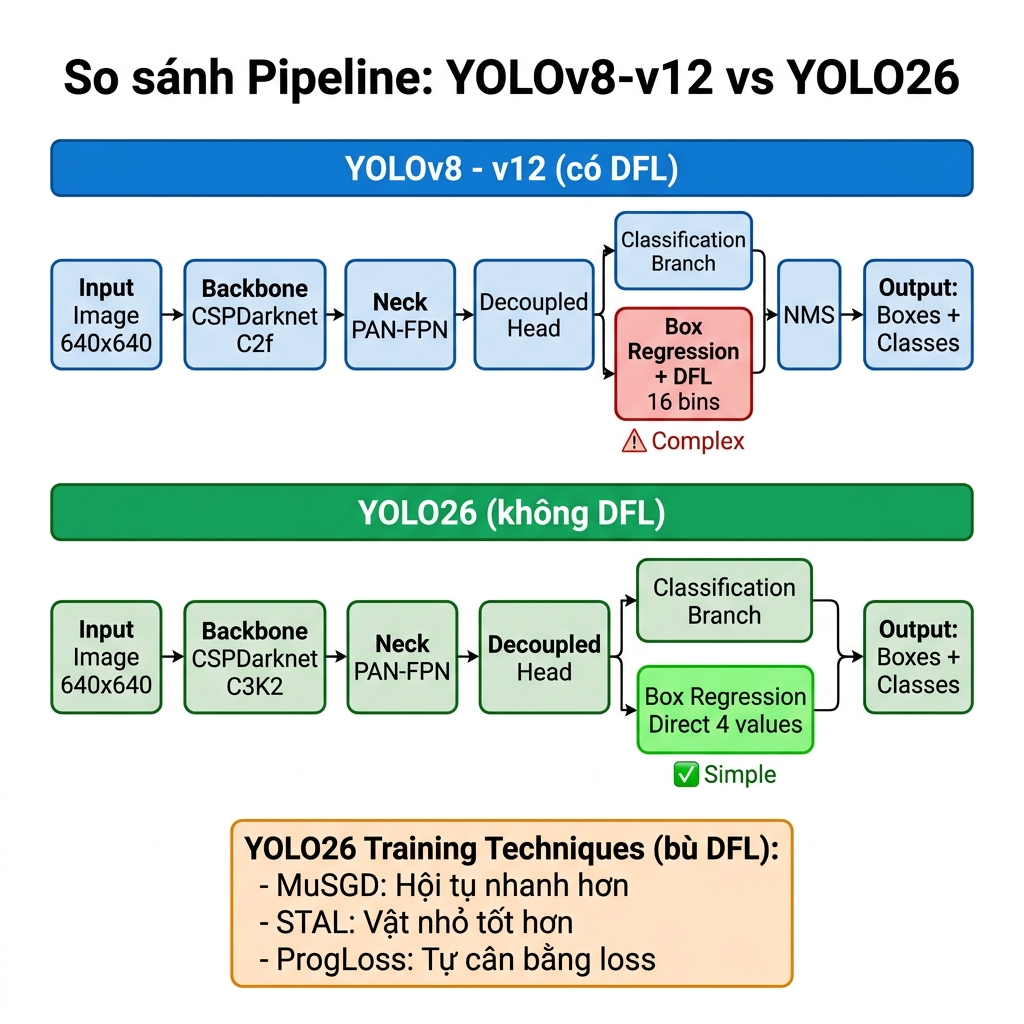
\includegraphics[width=\textwidth]{yolo26_pipeline.png}
\caption{So sánh pipeline: YOLOv8--v12 (có DFL, phức tạp) vs YOLO26 (không DFL, đơn giản hóa). YOLO26 bù bằng 3 training techniques: MuSGD, STAL, ProgLoss.}
\end{figure}
